\documentclass[../main.tex]{subfiles}

\begin{document}
\section{Results} \label{sec:results}
This section presents results obtained using the proposed calibration procedure with the Raspberry Pi camera array.

\subsection{Our implementation} \label{sec:calibration-implementation}
So far, we have found that the most effective calibration patterns are detailed images such as paintings (see figure~\ref{fig:calibration-pattern}).

We have positioned our Raspberry Pi camera array parallel to a TV displaying such a pattern (see figure~\ref{fig:calibration-setup}). This setup makes it easy to change the pattern while keeping the same reference plane distance.

\begin{figure}[H]
    \centering
    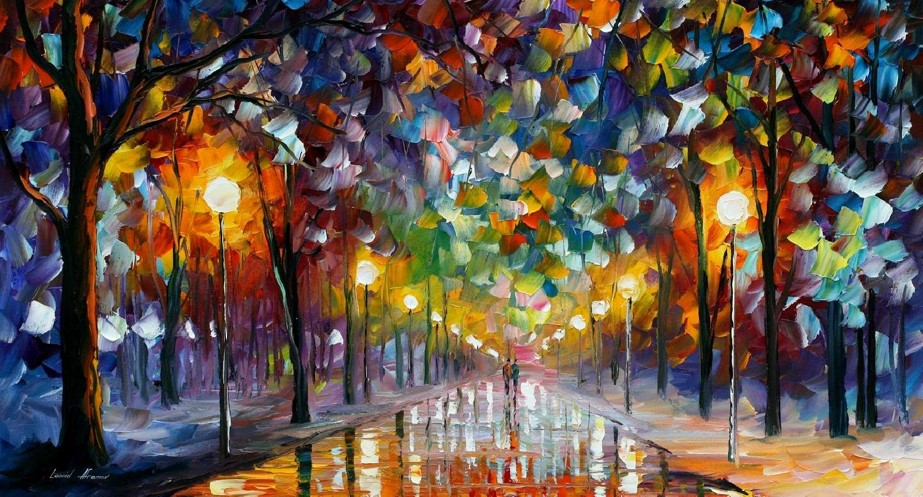
\includegraphics[width=\linewidth]{images/calibration-pattern}
    \caption{A calibration pattern that achieved good results for our camera. The image is of Leonid Afremov's \emph{Farewell to Anger}.}
    \label{fig:calibration-pattern}
\end{figure}

\begin{figure}[H]
    \centering
    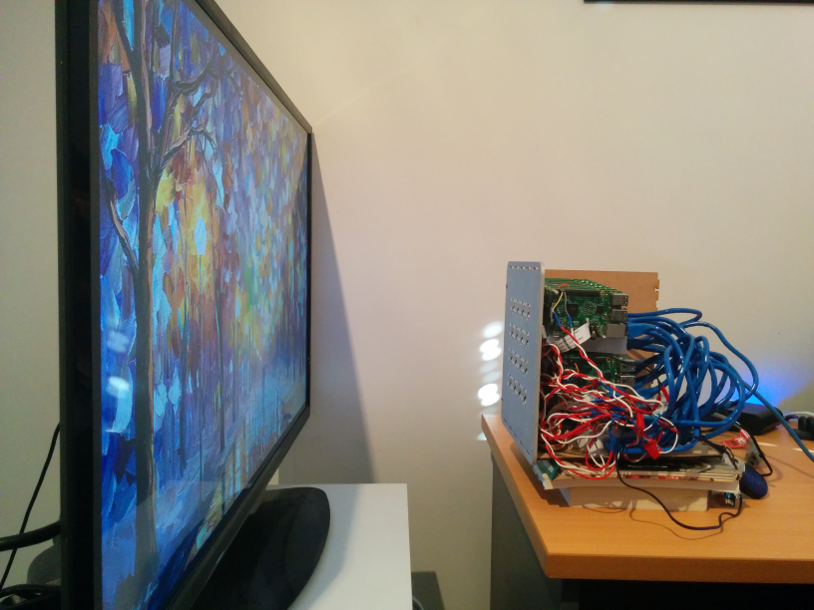
\includegraphics[width=0.85\linewidth]{images/calibration-setup}
    \caption{Our calibration setup. We have displayed our calibration image on a TV to ensure planarity, and aligned by visual inspection.}
    \label{fig:calibration-setup}
\end{figure}

\begin{figure}[H]
    \centering
    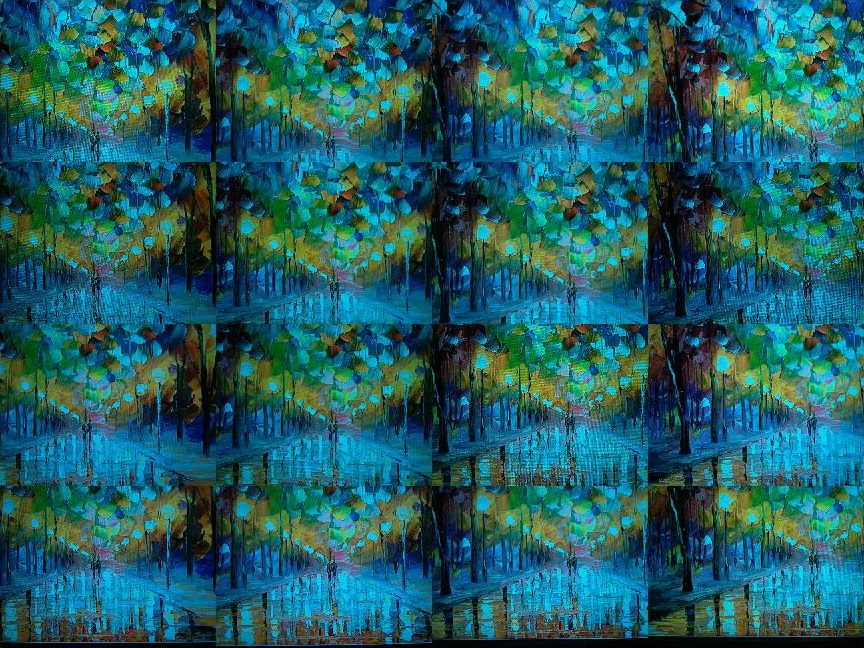
\includegraphics[width=0.85\linewidth]{images/calibration-set-painting}
    \caption{Mosaic of our calibration set}
    \label{fig:calibration-set-painting}
\end{figure}

\subsubsection{Approximate overlap}
For our 4x4 camera array, we have camera translations of $t=34.5$ mm, camera fields of view $\phi=(53.5^{\circ},41.41^{\circ})$, and a distance to the reference plane $d\approx300$ mm. Using basic geometry, and by assuming a precisely coplanar camera array and perpendicular viewing directions, we have:

\begin{equation} \label{eq1}
    \begin{split}
    \textrm{Projection width } P_x & = 2d \tan ( \frac{\phi_x} {2} ) \\
                                   & = 2\times300\times \tan ( \frac{53.5} {2} ) \\
                                   & = 302.424 \textrm{ mm}
    \end{split}
\end{equation}

\begin{equation} \label{eq2}
    \begin{split}
        x\textrm{ overlap} & = \frac{P_x-t}{P_x} \\
                           & = \frac{302.424 - 34.5}{302.424} \\ 
                           & = 88.59\%
    \end{split}
\end{equation}

So we have approximately $88.59\%$ overlap between camera views in the $x$ direction. Applying the same equations in the $y$ direction, we calculate approximately $84.78\%$ overlap.

\newpage
\subsection{Calibration accuracy} \label{sec:calibration-accuracy-result}
In section~\ref{sec:assessing-calibration}, we suggest that calibration accuracy can be tested by comparing the relative coordinates of features across rectified images. For a planar scene (such as the calibration set scene), perfect calibration is achieved when coordinates of features match precisely. A MATLAB implementation of this assessment procedure is provided in appendix~\ref{apx:rectified-set-accuracy}. 

We have calculated such pixel inconsistencies over multiple passes of the calibration procedure (see table~\ref{tbl:pixel-inconsistencies}). Multiple passes are achieved by estimating and transforming already rectified images successive times.
    
\begin{table}[H] 
    \centering
    \begin{tabular}{llll} 
        \textbf{\# of passes} & \textbf{\begin{tabular}[c]{@{}l@{}}x-inconsistency \\ (pixels)\end{tabular}} & \textbf{\begin{tabular}[c]{@{}l@{}}y-inconsistency \\ (pixels)\end{tabular}} & \textbf{\begin{tabular}[c]{@{}l@{}}Overall \\ inconsistency \\ (\%)\end{tabular}} \\
        1                     & 5.092                                                                        & 5.155                                                                        & 0.23                                                                                     \\
        2                     & 1.178                                                                        & 0.884                                                                        & 0.043                                                                                    \\
        3                     & 1.184                                                                        & 0.917                                                                        & 0.043                                                                                    \\
        4                     & 1.160                                                                        & 0.925                                                                        & 0.042                                                                            
        \end{tabular}
        \caption{Average pixel inconsistencies of reference plane features detected across rectified images}
        \label{tbl:pixel-inconsistencies} 
\end{table}

It is clear that after the second pass, we see significant diminishing returns. For our implementation, we have therefore opted for two passes. We achieve an overall final inconsistency of 0.043\%, from 0.23\% with only one pass (an improvement of a factor of $5.35$). Calibrated light fields can therefore be considered to be 99.957\% accurate in terms of their alignment and resultant focus.

It is critical to note that the average difference in feature positions does not necessarily correspond to reprojection error. Reprojection error is a common accuracy measure used in metric calibration procedures. Like Vaish et al's plane + parallax procedure, our procedure is non-metric, so we cannot calculate reprojection error. Vaish points out that non-metric procedures are not calculating the same intrinsic and extrinsic camera parameters, or making the same assumptions as metric calibration procedures \cite{vaish2004using}.

\subsection{Light field rendering}
Light fields can be rendered by shifting rectified images or \emph{light field slices} to a common depth, then adding the slices together to yield a single 2D output. Dansereau provides an implementation of this in his \emph{Light Field Toolbox} for MATLAB as \texttt{LFFiltShiftSum}. Light fields will initially need be loaded via \texttt{LFReadGantryArray}, which can take a rectified image set as input.

We can demonstrate the effectiveness of our calibration procedure by attempting to render a planar scene. We juxtapose an uncalibrated light field render with its rectified counterpart (see figure~\ref{fig:uncalibrated-vs-calibrated}). Note the increased clarity after rectification.

\begin{figure}[H]
    \centering
    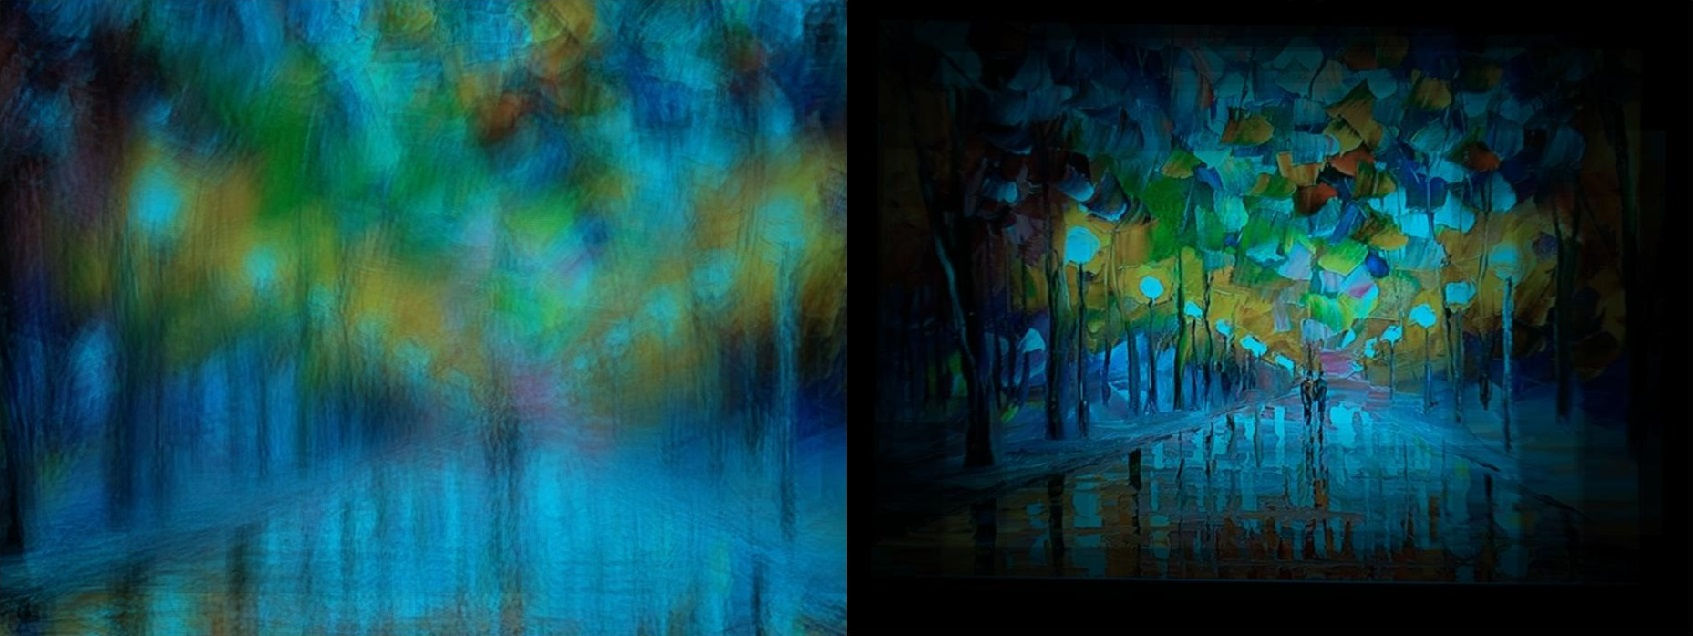
\includegraphics[width=\linewidth]{images/uncalibrated-vs-calibrated}
    \caption{Uncalibrated images rendered as a light field (left) vs. light field calibrated using our procedure (right).}
    \label{fig:uncalibrated-vs-calibrated}
\end{figure}

\newpage
\subsubsection{Synthetic aperture focusing and robustness to occlusion}
We can demonstrate our calibration procedure's appropriateness for synthetic aperture focusing applications by adjusting light field focus for non-planar scenes. A scene demonstrating synthetic focus of three depth levels is shown (see figure~\ref{fig:focus-levels}).

\begin{figure}[H]
    \centering
    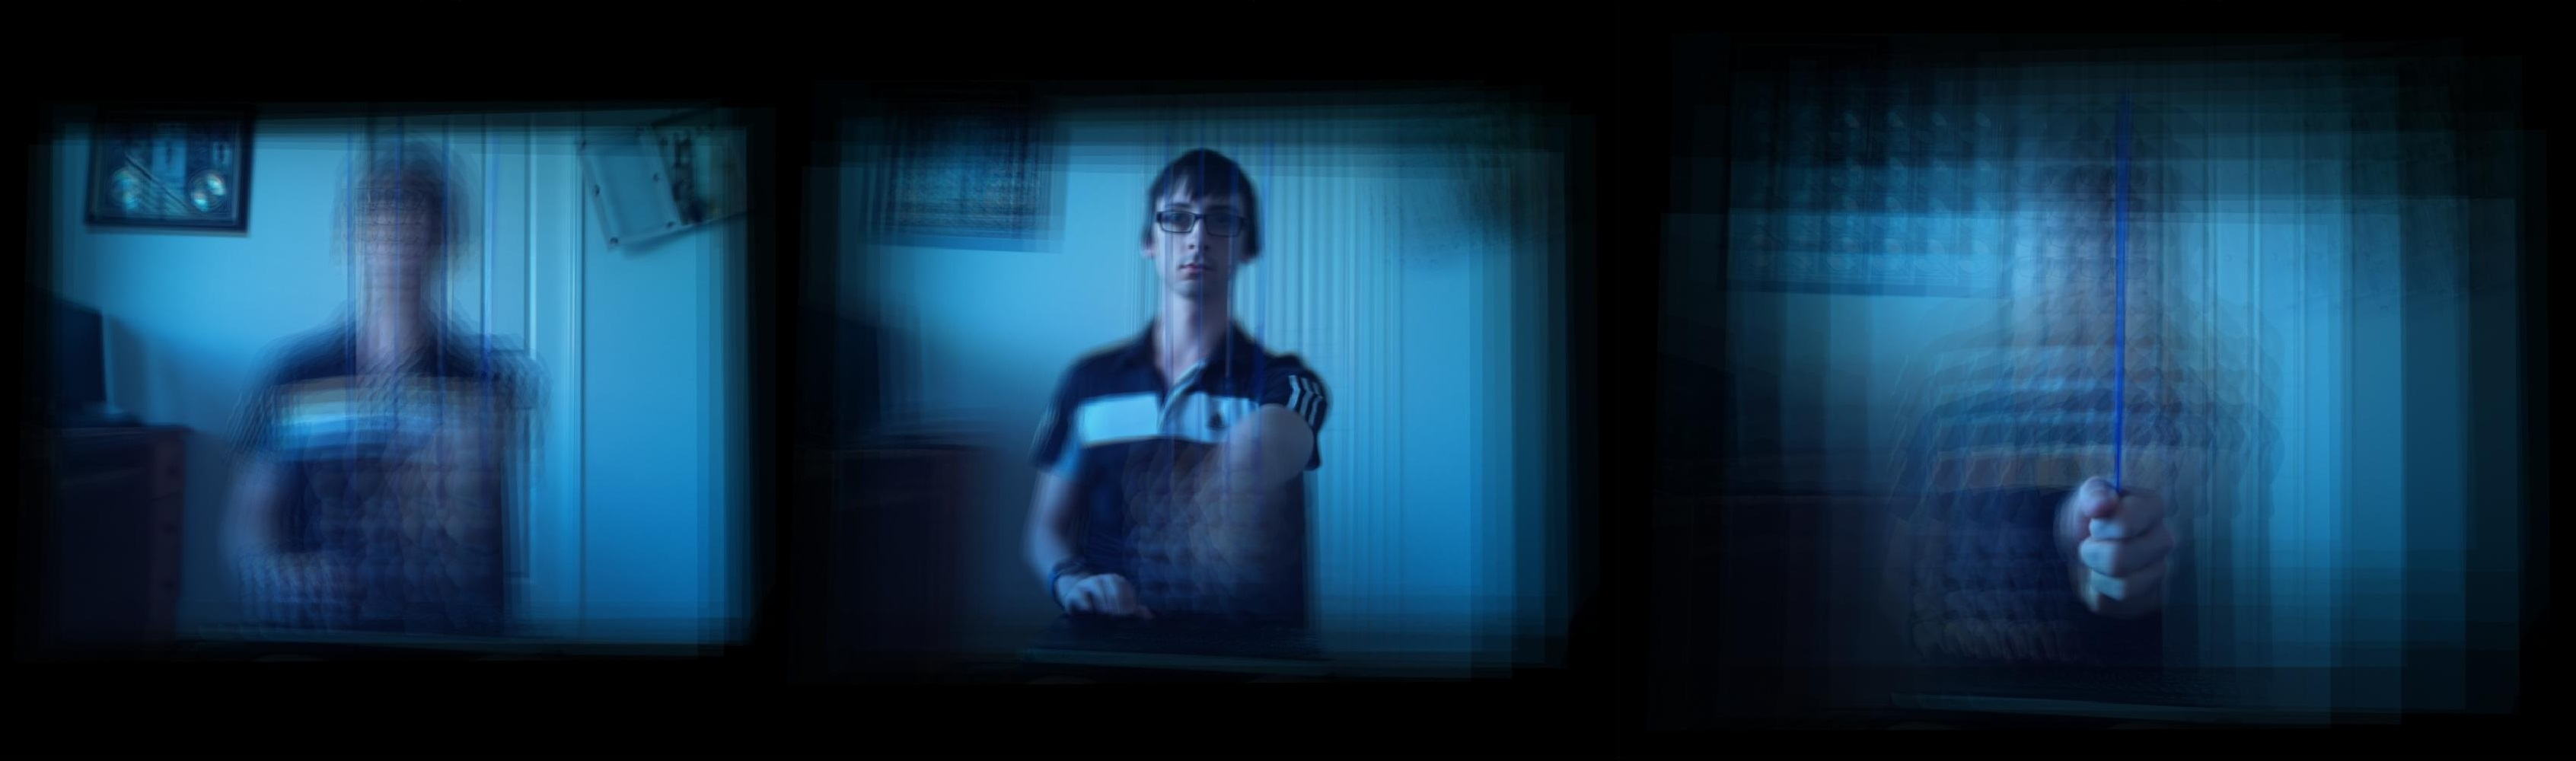
\includegraphics[width=\linewidth]{images/focus-levels}
    \caption{Three focus levels for a non-planar scene. Focus on backdrop (left), focus on person (middle), focus on fist holding ruler (right).}
    \label{fig:focus-levels}
\end{figure}

An application of particular interest in light field imaging is occlusion removal, which synthetic focusing can demonstrate robustness to. An example illustrating such robustness is shown (see figure~\ref{fig:robustness-to-occlusion} and figure~\ref{fig:occluder-set}).

\begin{figure}[H]
    \centering
    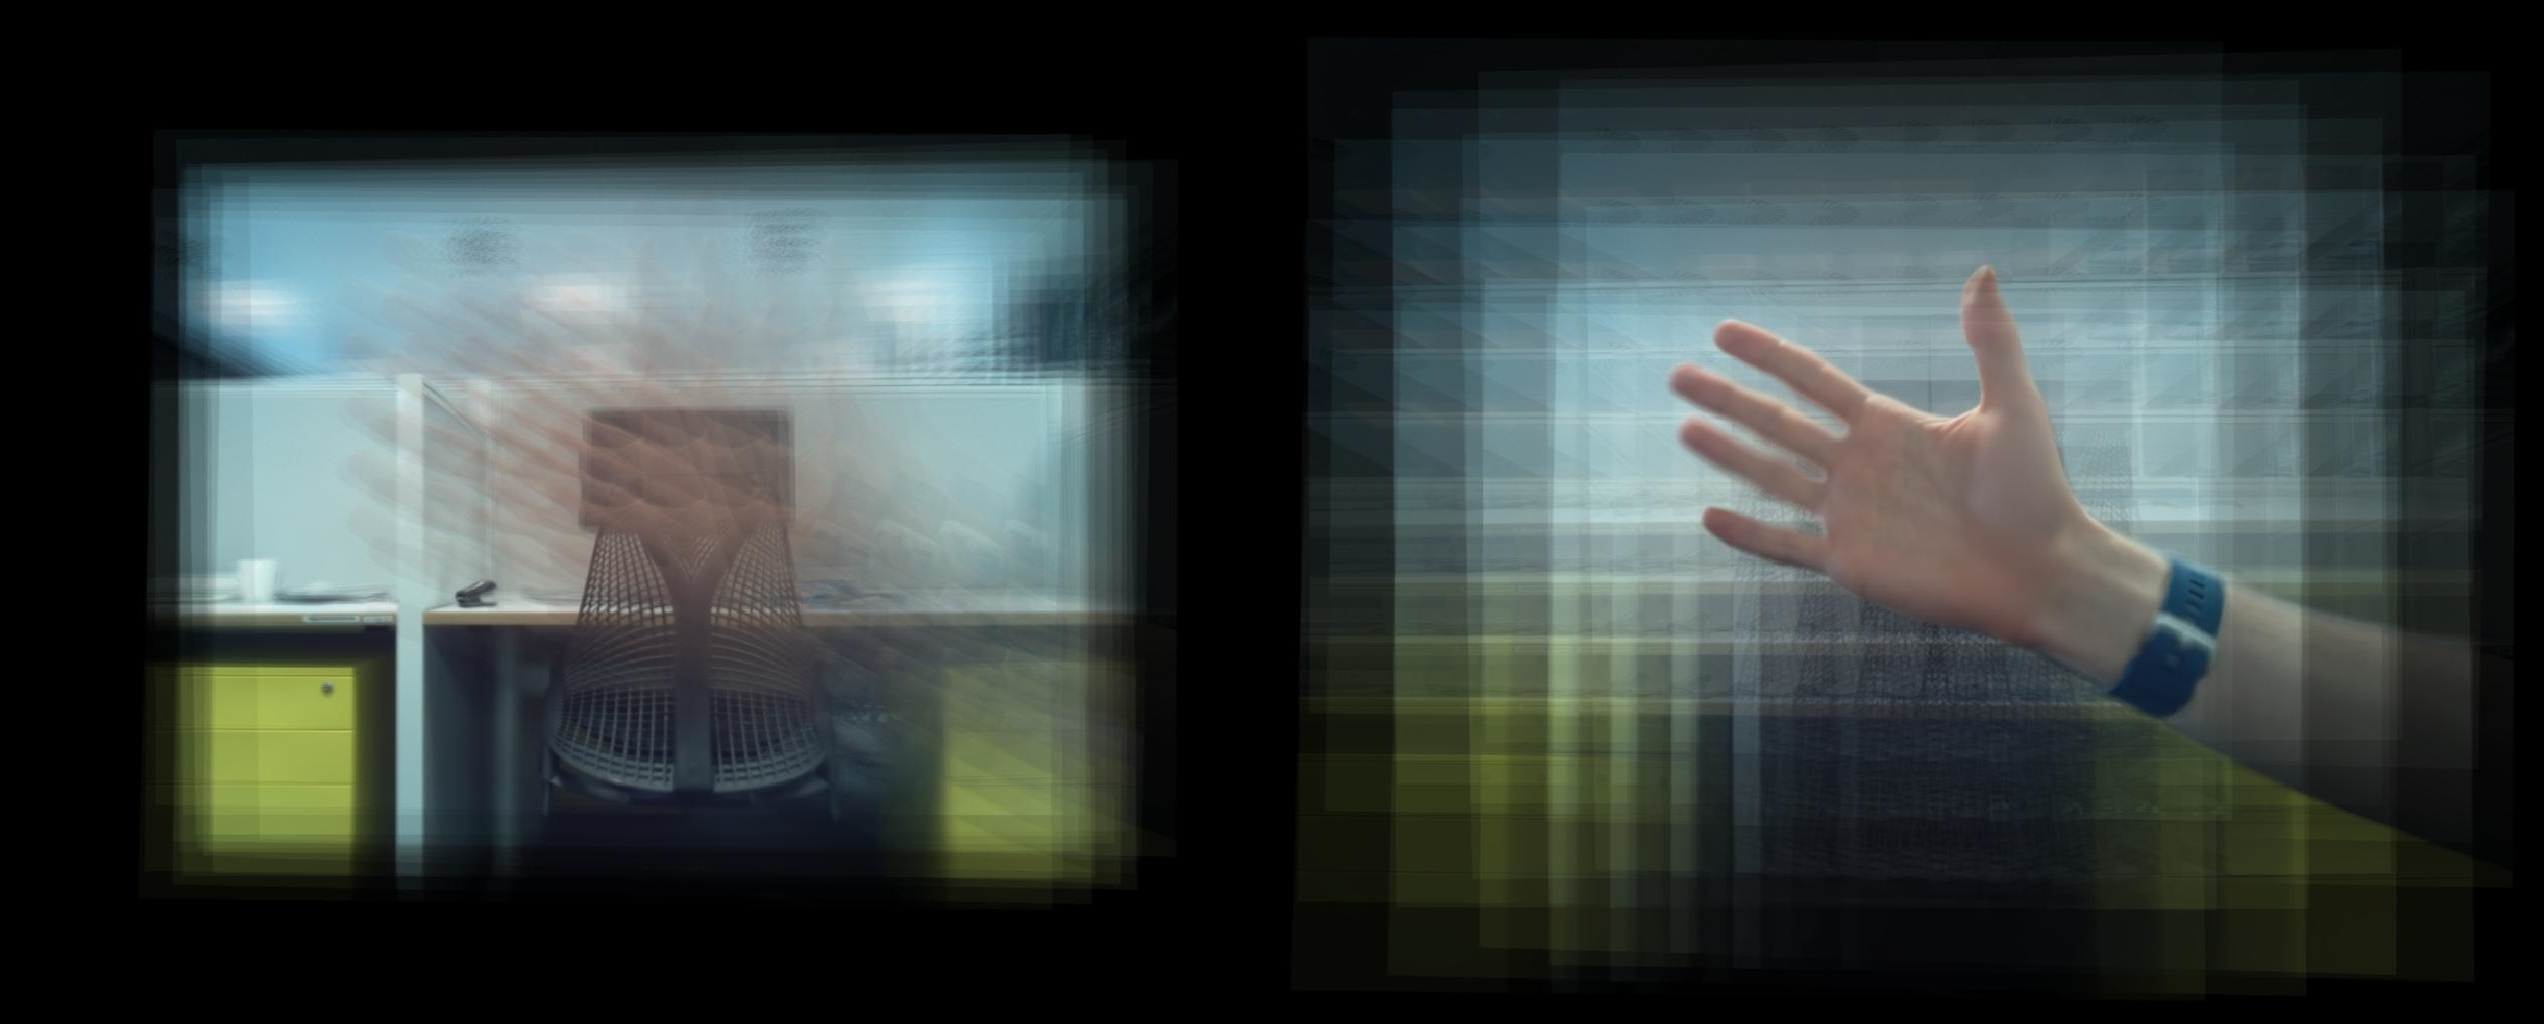
\includegraphics[width=\linewidth]{images/robustness-to-occlusion}
    \caption{Two focus levels of a non-planar scene with a significantly occluding hand. Focus on occluded area containing office chair and computer monitor (left) and focus on hand (right).}
    \label{fig:robustness-to-occlusion}
\end{figure}

\begin{figure}[H]
    \centering
    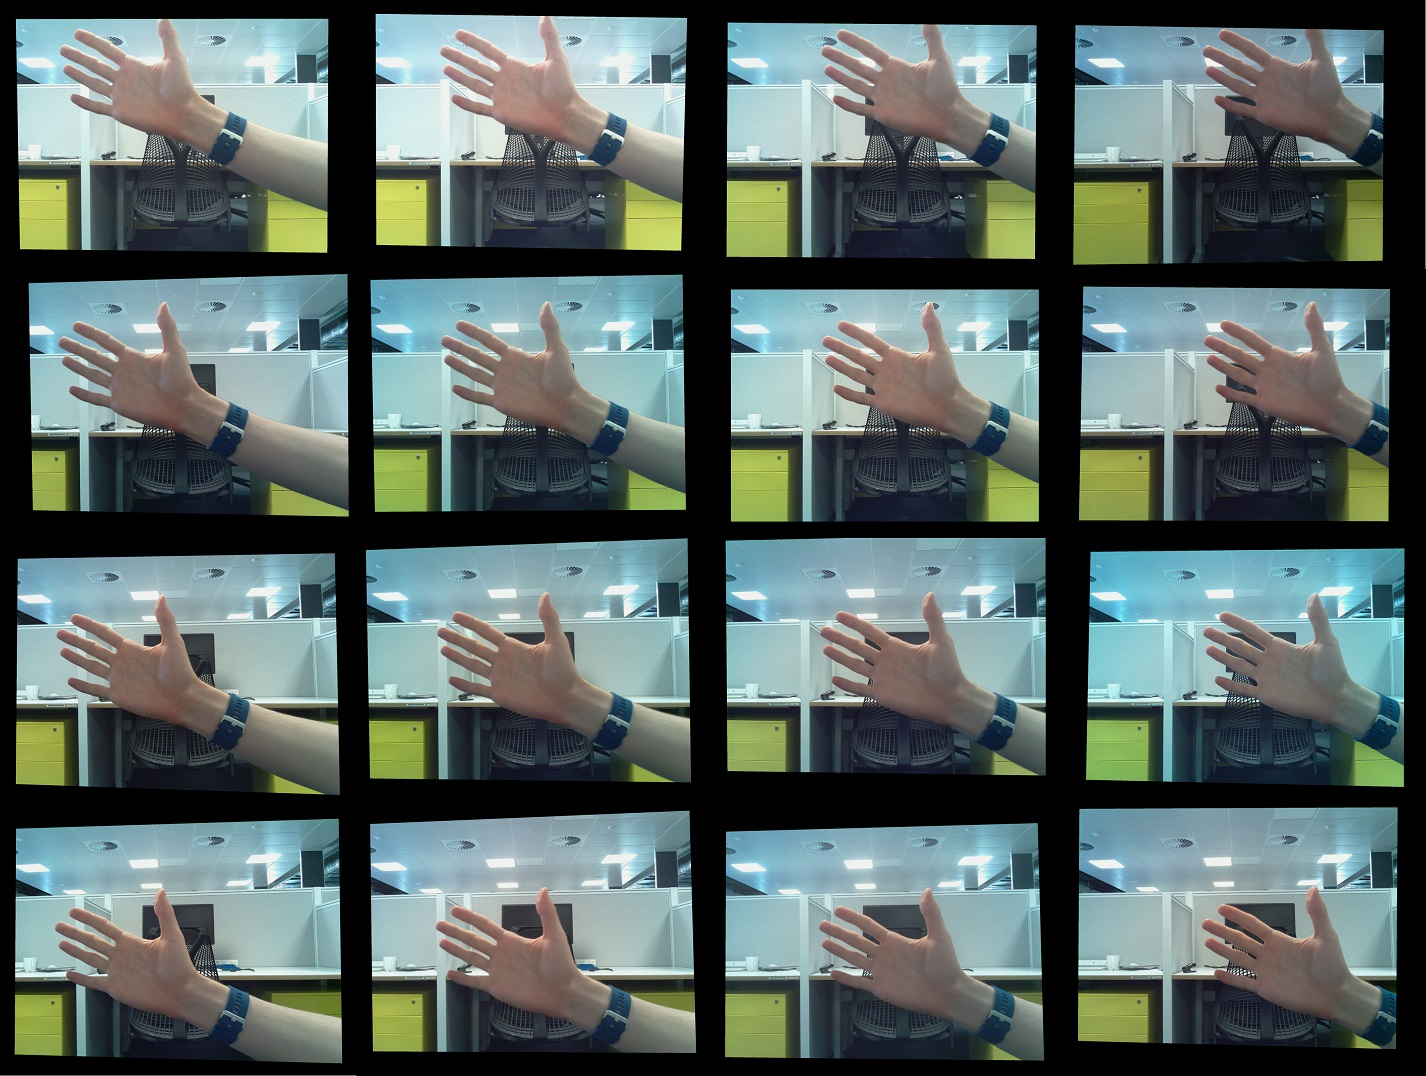
\includegraphics[width=\linewidth]{images/occluder-set}
    \caption{Rectified image set used to construct the rendered light fields in figure~\ref{fig:robustness-to-occlusion}. Note that in each camera view, a significant portion of the monitor or the office chair is occluded.}
    \label{fig:occluder-set}
\end{figure}

\newpage
\subsubsection{Light field video}
Light field video is another area of particular interest to our applications, and very little work has been done in light field imaging that exploits the temporal axis. We have been able to construct light field video by extracting each frame of video, and thus construct a light field for each frame.

The Raspberry Pi camera array has been able to capture synchronised video with $<1$ centisecond of synchronisation disparity. This has been achieved by recording a stopwatch across all cameras and commanding video capture by sending synchronised SSH (see figure~\ref{fig:video-sync}).

\begin{figure}[H]
    \centering
    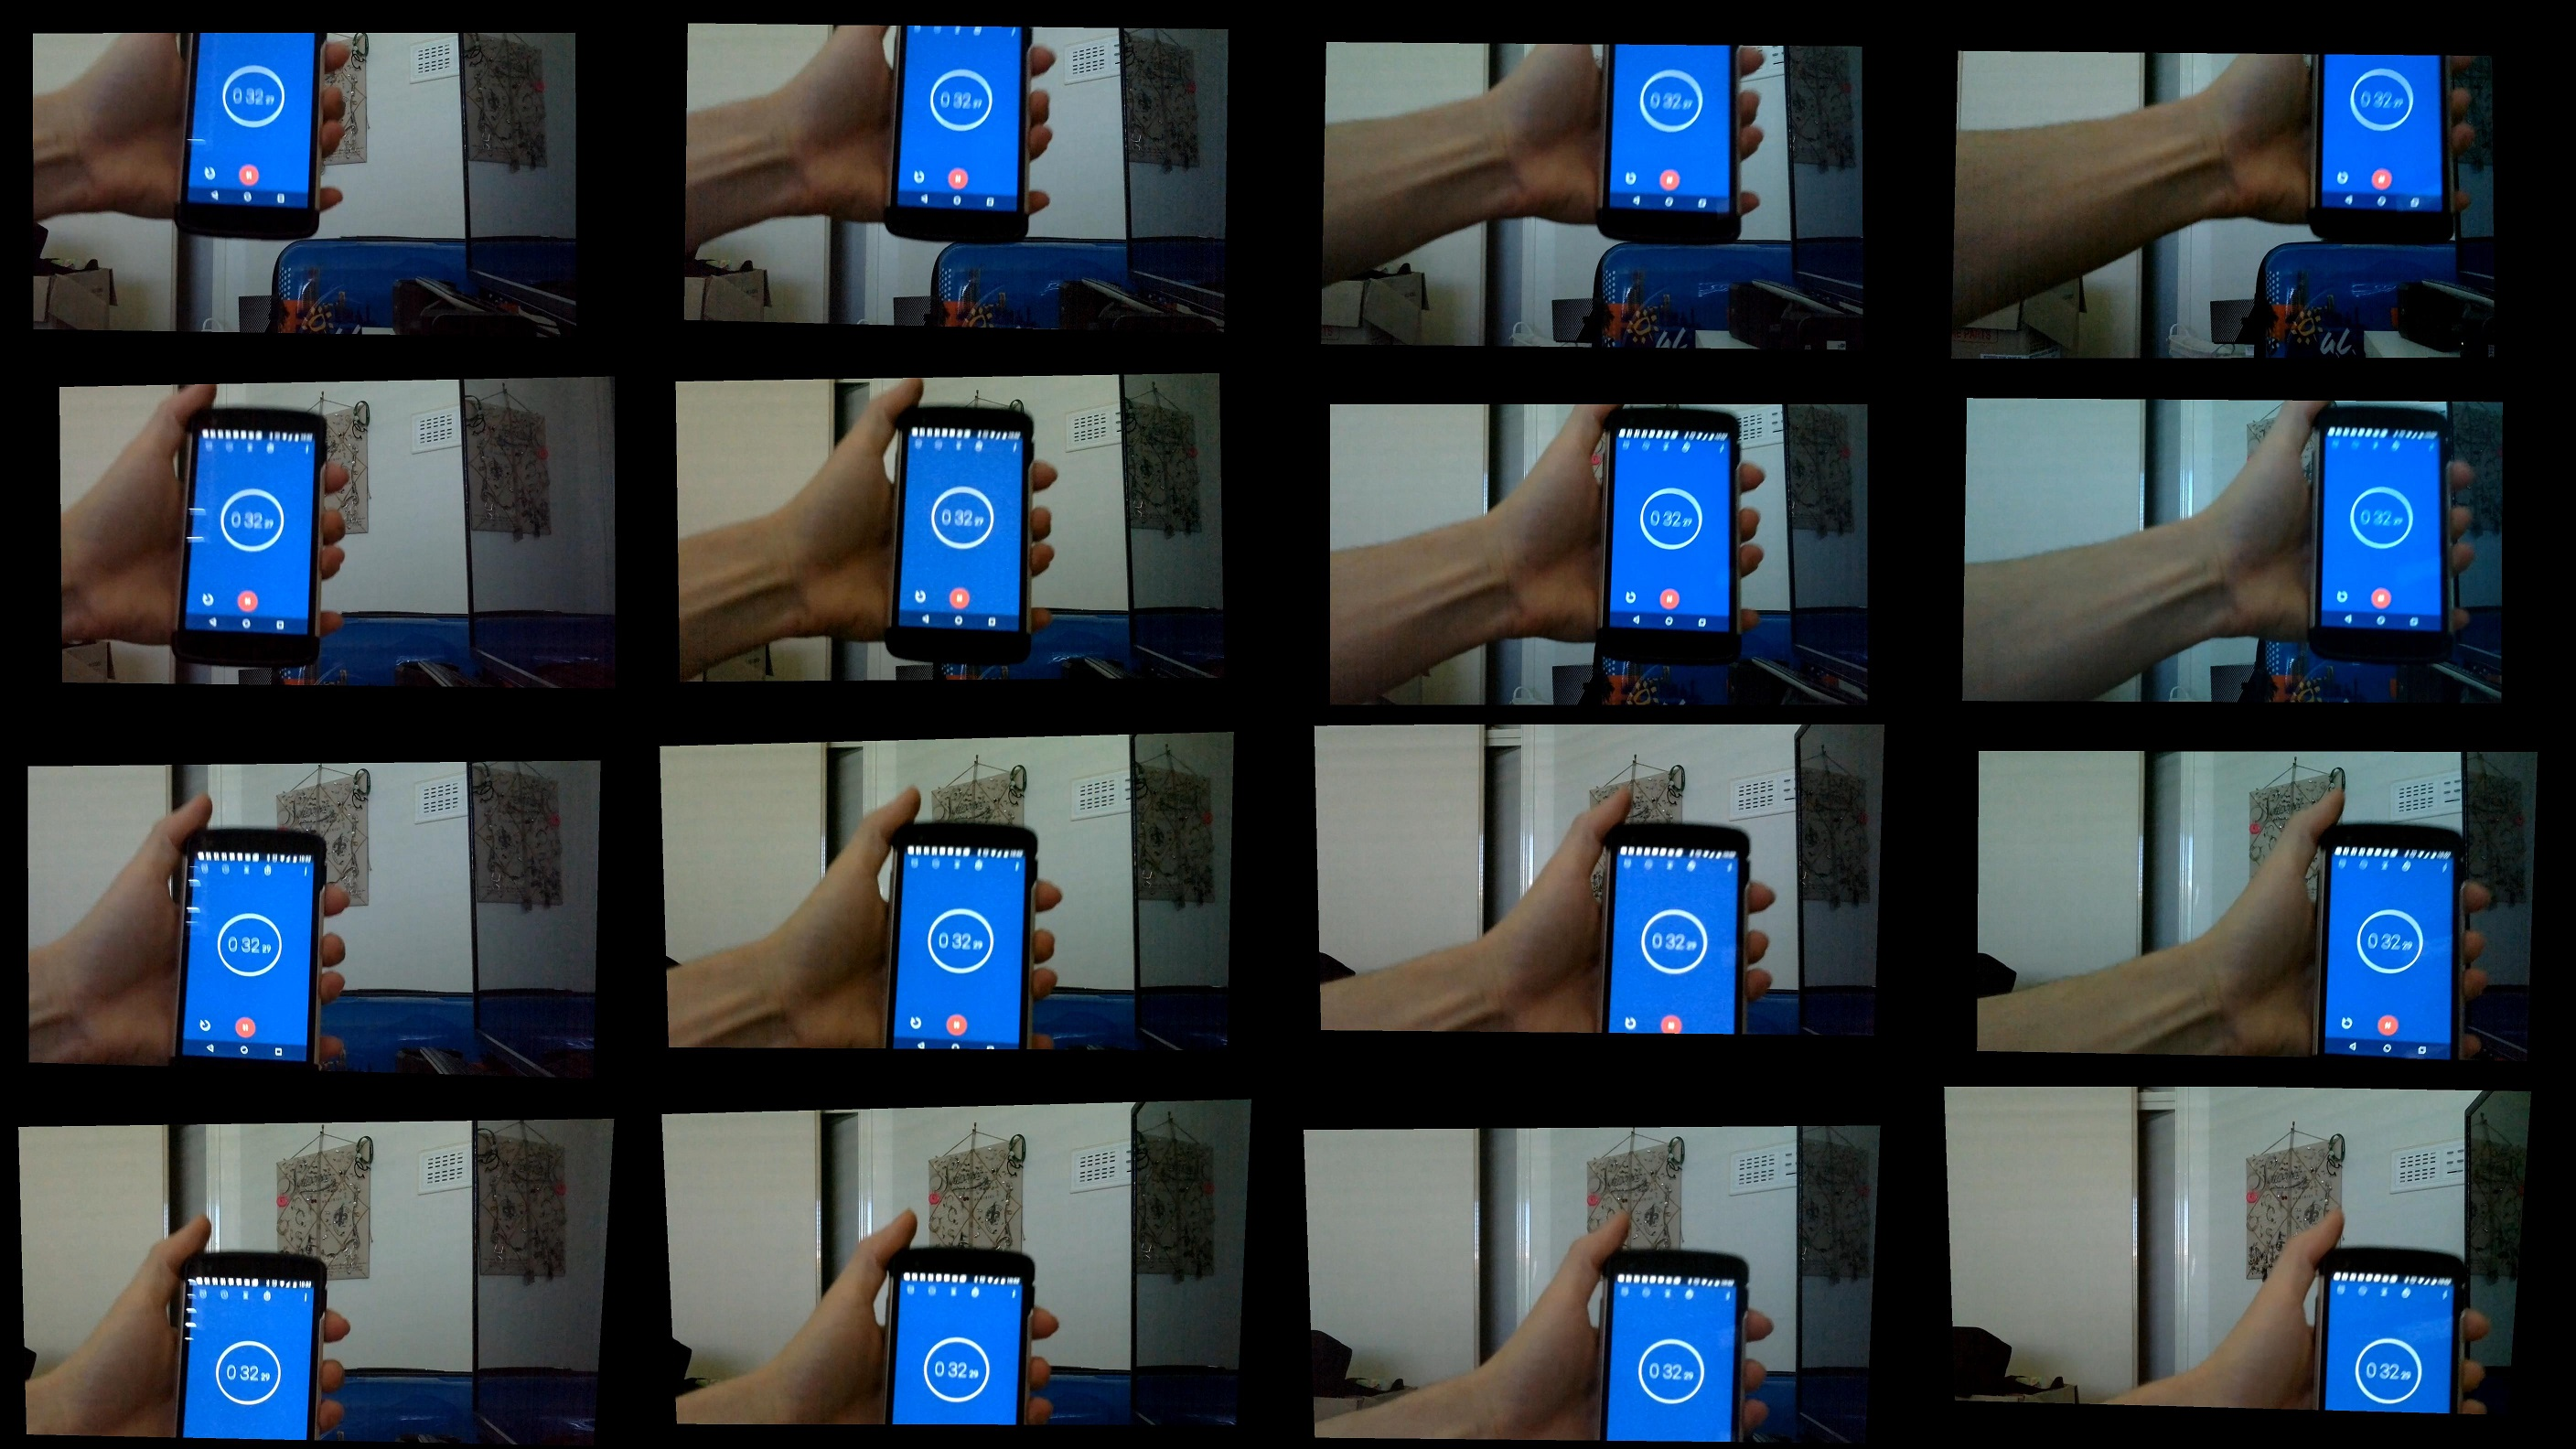
\includegraphics[width=\linewidth]{images/video-sync}
    \caption{Recorded video has been shown to be synchronised to less than one centisecond. The camera modules exhibit  significant motion blur over smaller timespans due to the shutter speed.}
    \label{fig:video-sync}
\end{figure}

Additionally, we have demonstrated light field video that adjusts focus, to demonstrate aperture focusing with moving occluders (see figure~\ref{fig:video-frames}).

\begin{figure}[H]
    \centering
    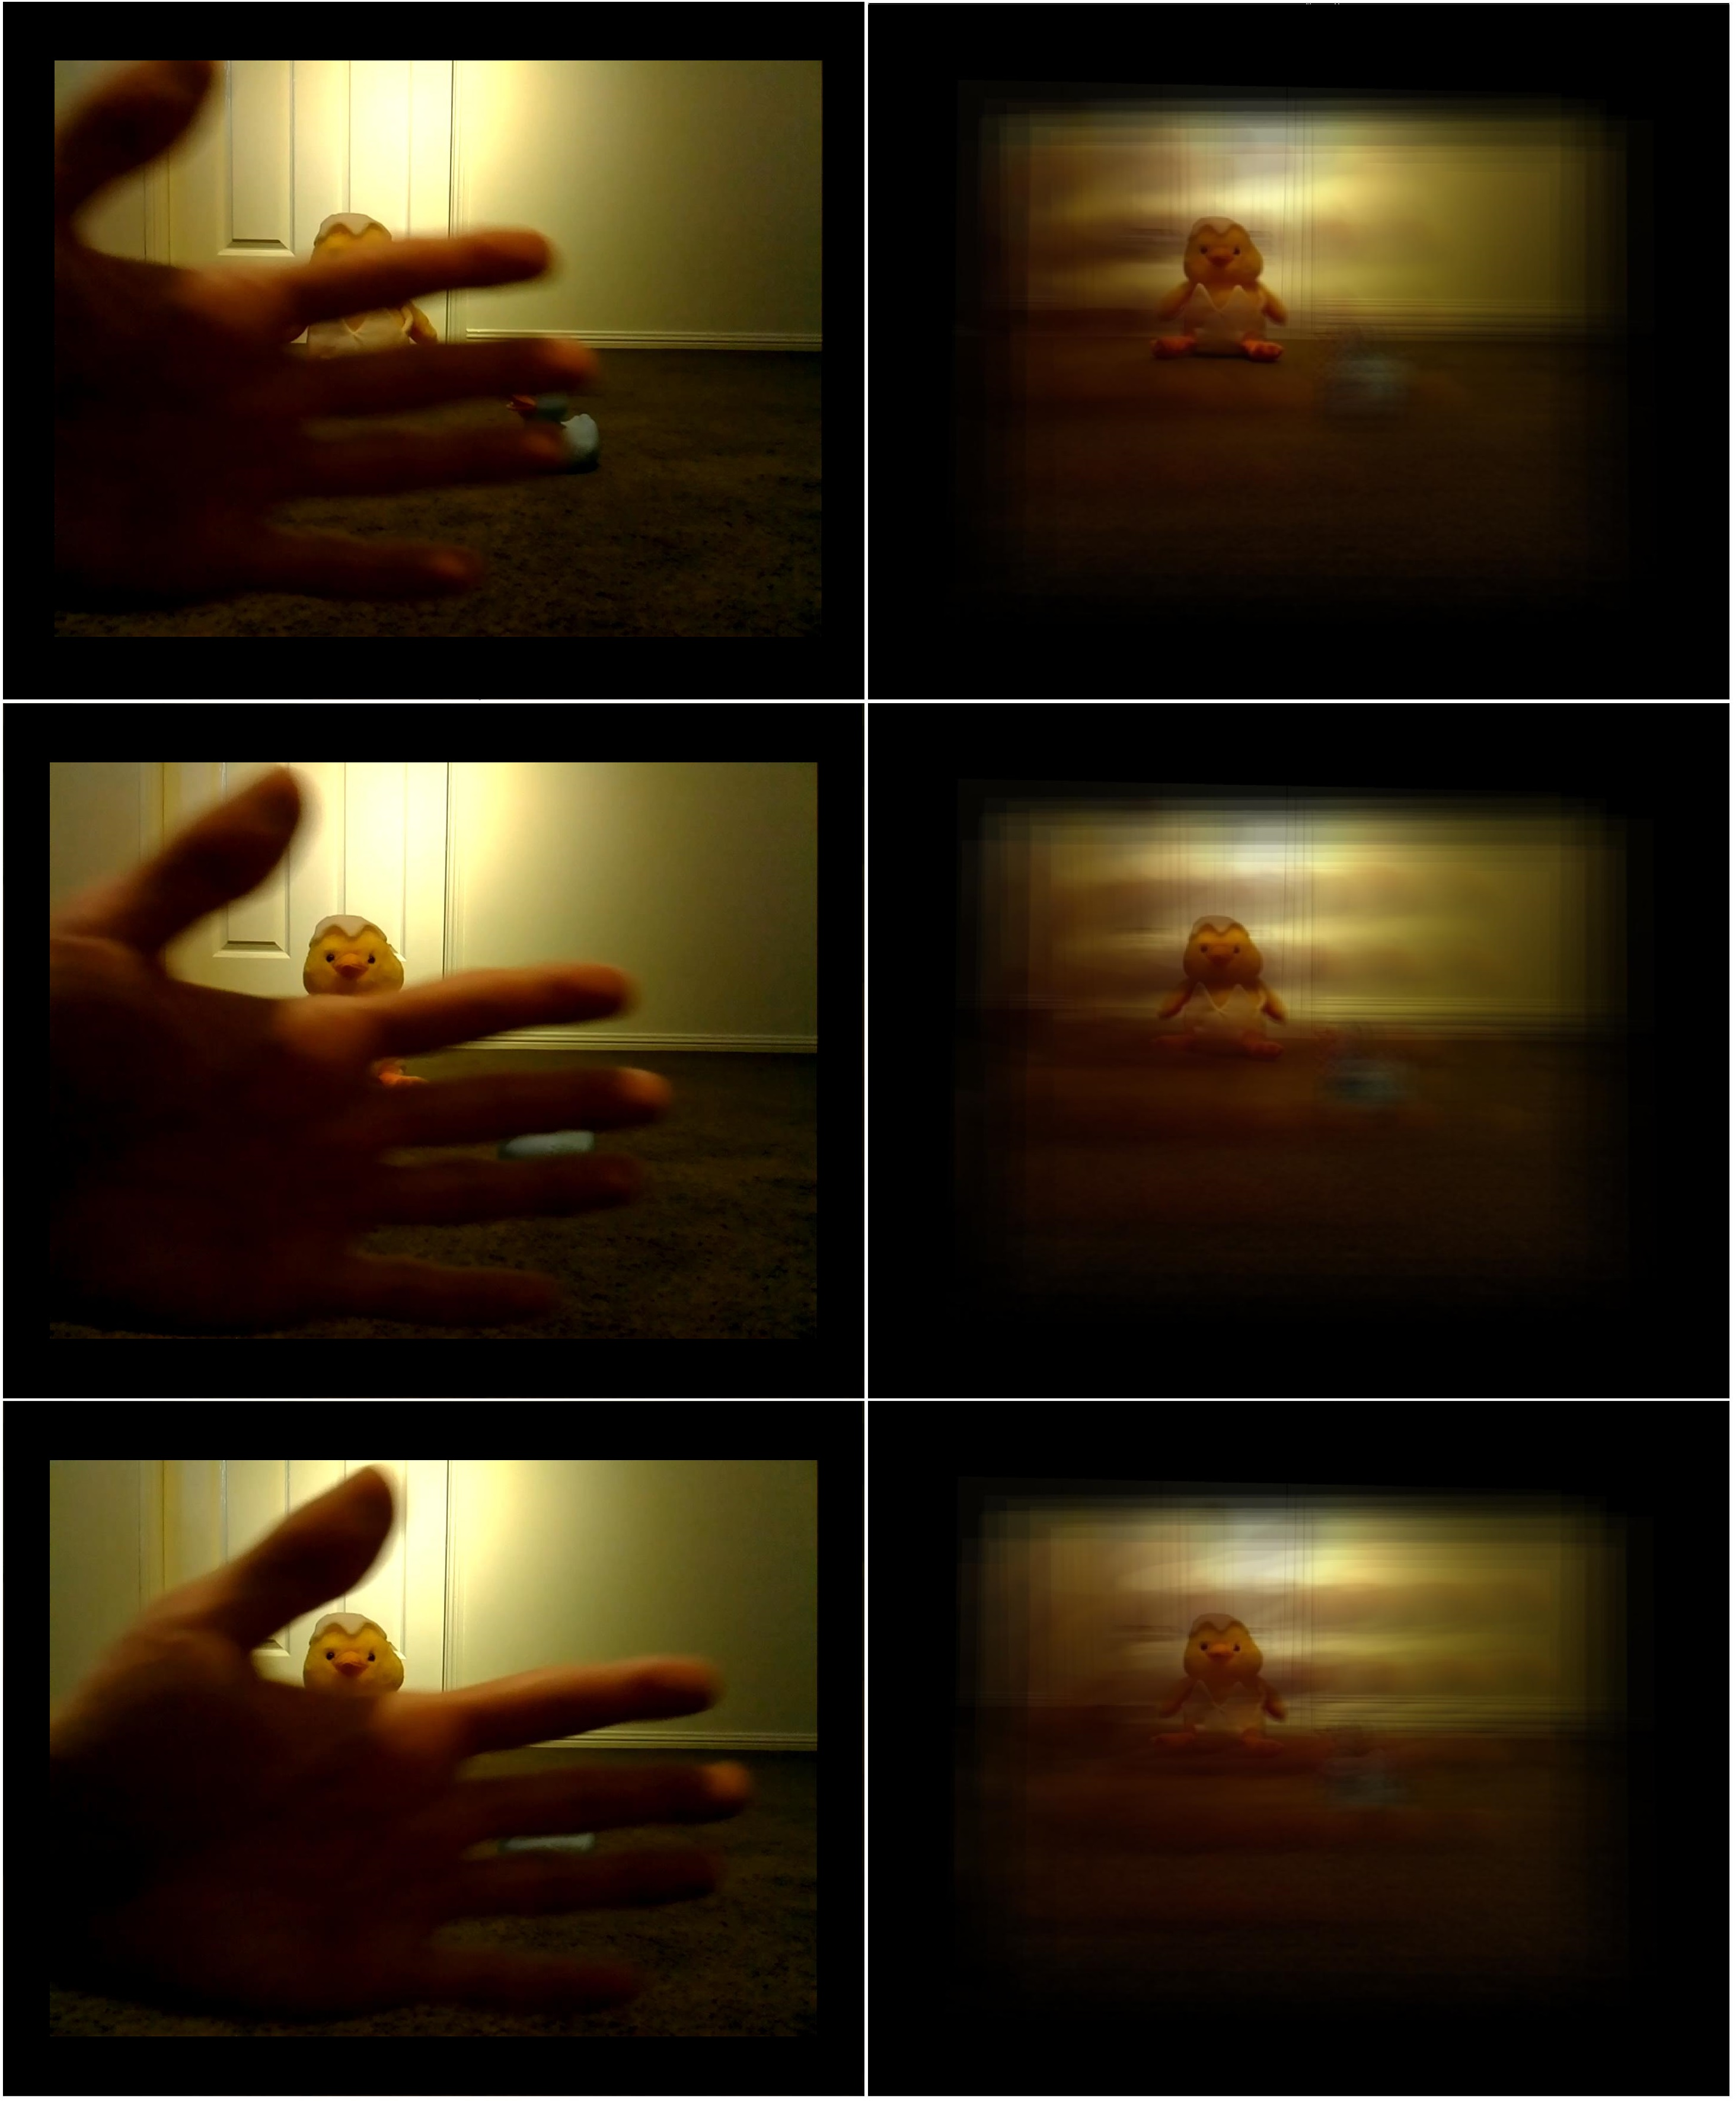
\includegraphics[width=\linewidth]{images/video-frames}
    \caption{Three frames of video have been selected. The left-hand images show the frames from raw video captured by one of our camera modules. The right-hand images show the same frames, but rendered as a light field - the focus is on the stuffed toy.}
    \label{fig:video-frames}
\end{figure}

\newpage

\end{document}